\documentclass[10.5pt]{config}
% 本实验报告采用 署名-相同方式共享 4.0 国际许可协议 (CC BY-SA 4.0)
\usepackage{multirow}
\usepackage{wrapfig}
\usepackage{setspace}
\usepackage{titlesec}
\usepackage{ctex}
\usepackage{graphicx} % 用于插入图片
\usepackage{float}    % 用于控制图片位置
\usepackage{makecell}

\titleformat{\subsubsection}[block]  % 设置为块级标题（自动换行）
{\normalfont\bfseries}{\thesubsubsection}{1em}{} 
\titlespacing*{\subsubsection}{1.5em}{3.25ex}{1.5ex}  % 调整缩进：左缩进2em
\setstretch{1.5}

% --- 请在这里填写您的个人信息 ---
\major{机械工程} % 专业
\name{韩颂义}
\partner{} % 签名栏
\stuid{3240104198}
\date{3.5}
\lab{东3-208}
\grades{}
\course{电工电子学实验}
\instructor{季瑞松} % 指导老师
\exptype{基础实验} % 实验类型
\expname{基本电量测量和常用仪表使用} % 实验名字


\begin{document}

\makeheader % 首页头部

\section{实验目的和要求}
\begin{enumerate}
    \item 理解掌握基尔霍夫定律。
    \item 了解电工电子综合实验台上仪器仪表的布局，掌握直流电流源、直流电压表、直流电流表的使用方法。
    \item 掌握稳压电源的使用方法。
    \item 掌握数字式万用表的使用方法。
    \item 掌握电压表内阻、电流表内阻的测量方法。
    \item 了解电压表内阻和电流表内阻对测量准确度的影响。

\end{enumerate}

\section{实验内容和原理}
\subsection{实验原理}

\textbf{基尔霍夫定律}

基尔霍夫定律包括电压和电流两个定律，是电路的基本定律。

基尔霍夫电压定律是指在任何电路中，形成任何一个回路的所有支路沿同一循行方向电压的代数和在任何时刻都等于零。其数学表达式为
$$\sum u = 0$$

基尔霍夫电流定律是指在任何电路中，任何结点上的所有支路电流的代数和在任何时刻都等于零。其数学表达式为
$$\sum i = 0$$

\textbf{电量测量}


通常用“分压法”来测量电压表的内阻（图1）。将$R$值电阻与电压表串联后接到电压源上。测量时，先闭合开关 S，此时电压表的读数即为$U_S$；然后断开 S，此时电压表读数为$U_V$。由基尔霍夫电压定律，有
$$U_S = U_V + U_R$$
而
$$U_V = \frac{R_V}{R + R_V} U_S$$
故电压表内阻为
$$R_V = \frac{U_V}{U_S - U_V} R$$
为尽可能提高测量精度，通常将电路中的电阻采用精密可调电位器。测量时，先合上开关 S，调节$U_S$至电压表尽量接近满量程；打开 S，调节电位器，使得电压表读数为$U_S / 2$，则由分压原理可知电压表内阻$R_V = R$。

\begin{figure}[H]
    \centering
    % 宽度为页面40%，保持宽高比
    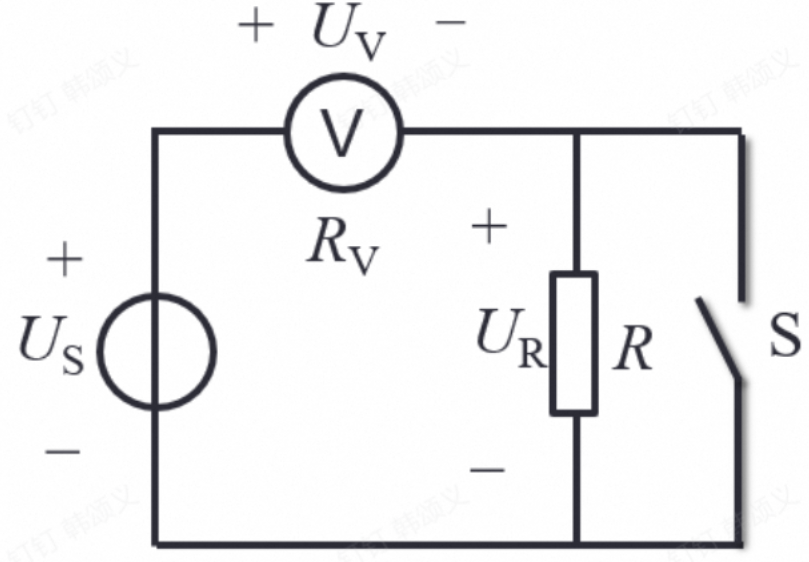
\includegraphics[width=0.3\textwidth, keepaspectratio]{figures/fenya.png}
    \caption{分压法}
    \label{fig:voltmeter_resistance}
\end{figure}

测量电流表的内阻通常用“分流法”（图2）。将一个$R$值电阻与电流表并联后接到电流源上，断开开关 S，此时电流表的读数即为$I_S$。然后闭合 S，此时电流表读数为$I_A$。由基尔霍夫电流定律，有
$$I_S = I_A + I_R$$
而
$$I_A = \frac{R}{R + R_A} I_S$$
故电流表内阻为
$$R_A = \frac{I_S - I_A}{I_A} R$$

为尽可能提高测量精度，通常将电路中的电阻采用精密可调电位器。测量时，先断开开关 S，调节$I_S$至电流表尽量接近满量程；闭合 S，调节电位器，使得电流表读数为$I_S / 2$，则由分流原理可知电流表内阻$R_A = R$。

\begin{figure}[H]
    \centering
    % 宽度为页面40%，保持宽高比
    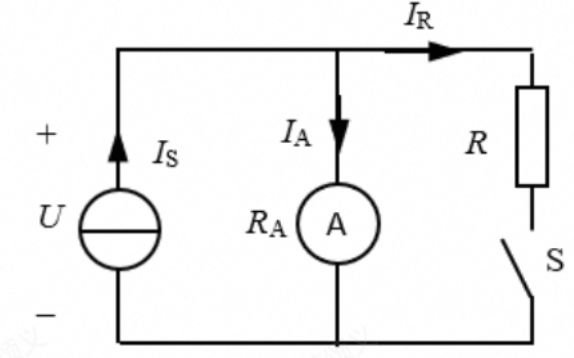
\includegraphics[width=0.3\textwidth, keepaspectratio]{figures/fenliu.png}
    \caption{分流法}
    \label{fig:voltmeter_resistance}
\end{figure}


\textbf{误差分析}

必须注意选择适当的仪表量程以减小方法误差。
即便是合格的测量仪表本身也存在着一定的误差，称为仪器误差。为了减小这种仪器误差，通常用同一只电压表来测量电路中的多处电压。

\section{主要仪器设备}
\begin{enumerate}
    \item 电工电子综合实验台。
    \item 数字式万用表。
    \item 稳压电源。
    \item 电阻元件、十进制电阻箱。
\end{enumerate}

\section{操作方法和实验步骤}

\subsection{直流电压、电流和电阻的测量}

\begin{enumerate}
    \item \textbf{电阻测量：} 选取标称值为 $330\Omega$ 和 $620\Omega$ 的两只电阻，在未接入电路的情况下，使用万用表电阻挡分别测量其实际阻值 $R_1$ 和 $R_2$ 并记录。
    \item \textbf{电路连接：} 按照图3将稳压电源、电流表和两只电阻串联连接。
    \item \textbf{电压测量：} 开启稳压电源，将其输出电压调节为恒定的 $U = 12\text{V}$。使用万用表直流电压挡，分别测量总电压 $U$ 以及两个电阻两端的电压 $U_1$ 和 $U_2$。
    \item \textbf{电流测量：} 使用直流电流表测量电路中的电流 $I$。
    \item \textbf{记录数据：} 将上述测得的电压、电流值记录在表1中，以验证 $U = U_1 + U_2$。
\end{enumerate}

\begin{figure}[H]
    \centering
    % 宽度为页面40%，保持宽高比
    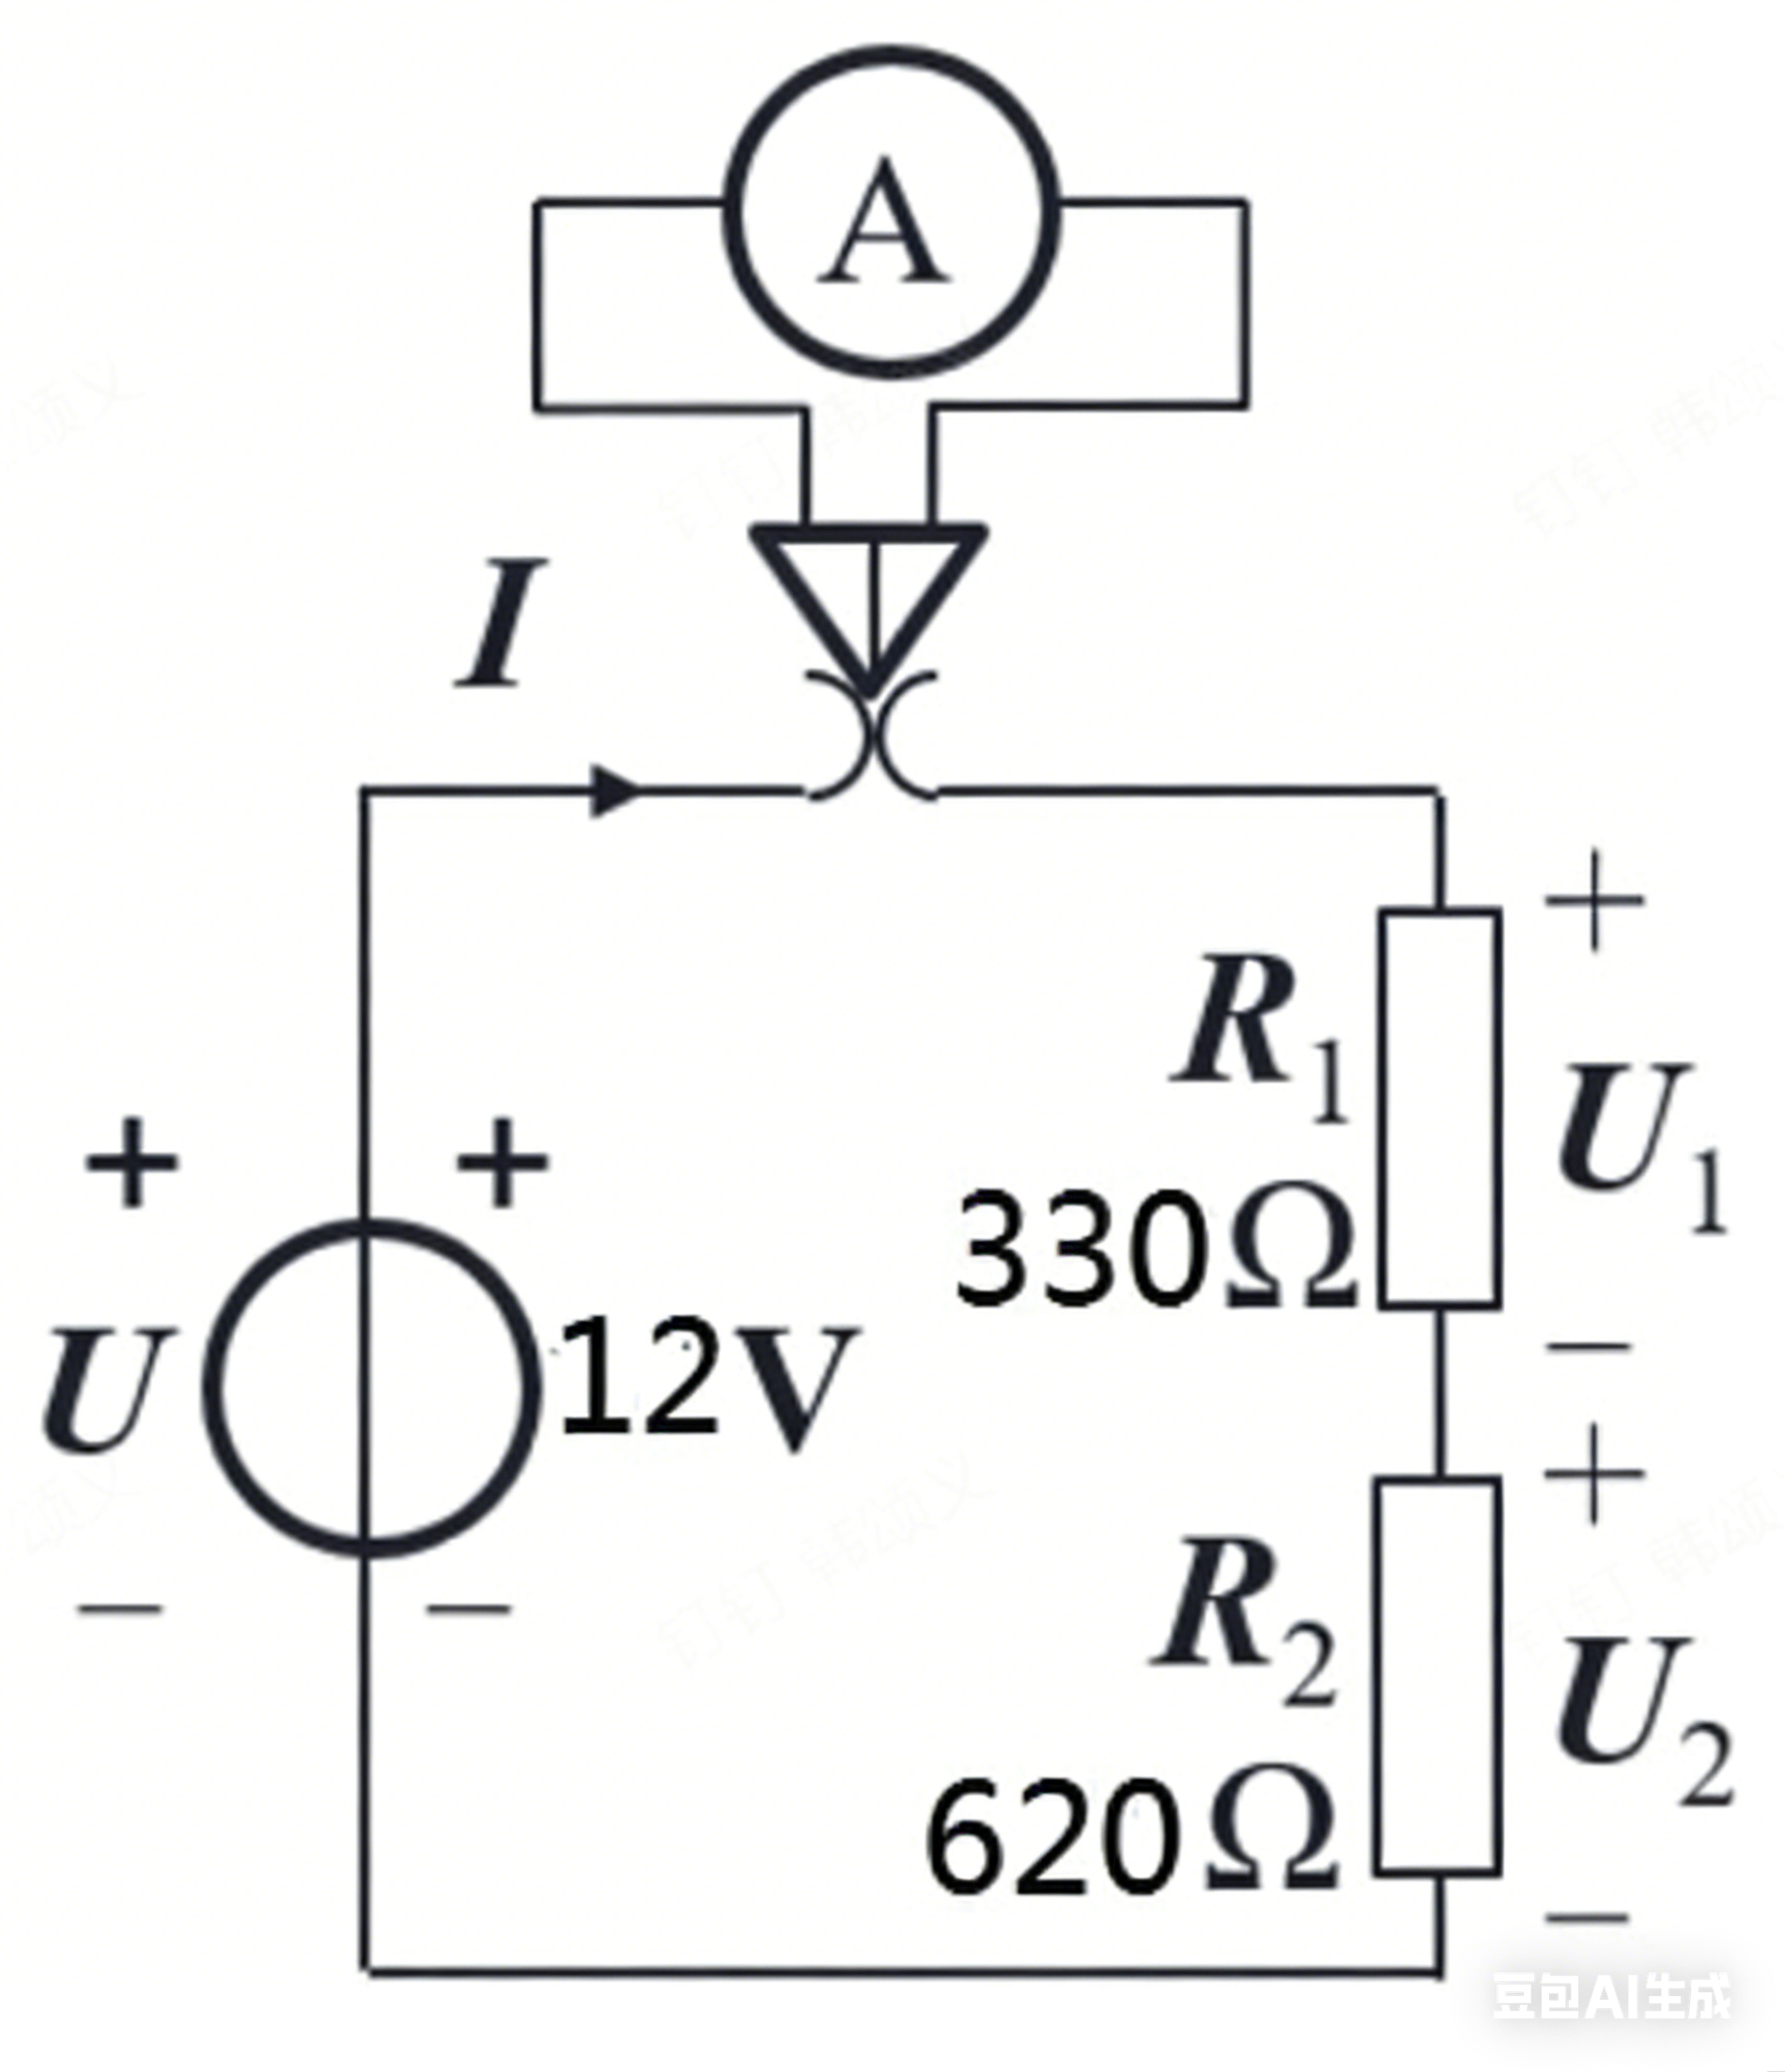
\includegraphics[width=0.3\textwidth, keepaspectratio]{figures/diyi.png}
    \caption{分流法}
    \label{fig:voltmeter_resistance}
\end{figure}

\subsection{电压表、电流表内阻的测量}

\subsubsection*{2.1 电压表内阻的测量（分压法）}
\begin{enumerate}
    \item \textbf{电路连接：} 按图1连接电路，将电阻 $R$ 与待测电压表串联后接入稳压电源。
    \item \textbf{闭合测量：} 闭合开关 S（此时电阻 $R$ 被短路），记录此时电压表的读数，记为 $U_S$。
    \item \textbf{断开测量：} 断开开关 S（此时电阻 $R$ 与电压表串联），记录此时电压表的读数，记为 $U_V$。
    \item \textbf{计算内阻：} 利用公式 $R_V = \frac{U_V}{U_S - U_V} R$ 计算电压表内阻，并将数据填入表2。\textit{（注：若使用半偏法，则调节可调电阻使 $U_V = U_S / 2$，此时 $R_V = R$）}。
\end{enumerate}

\subsubsection*{2.2 电流表内阻的测量（分流法）}
\begin{enumerate}
    \item \textbf{电路连接：} 按图2连接电路，将十进制电阻箱 $R$ 与待测电流表并联。将稳压电源设置为恒流源模式。
    \item \textbf{断开测量：} 先断开开关 S（电流全部流经电流表），调节恒流源输出，使电流表指针接近满量程，记录此时电流表读数为 $I_S$。
    \item \textbf{闭合调节：} 闭合开关 S，调节十进制电阻箱的旋钮，使电流表的读数下降到接近 $I_S / 2$ 的位置，记为 $I_A$。
    \item \textbf{阻值测量与计算：} 断开电路，用万用表电阻挡测量此时十进制电阻箱的输出阻值 $R$。利用公式 $R_A = \frac{I_S - I_A}{I_A} R$ 计算电流表内阻，并记录入表3。
\end{enumerate}



\section{实验数据记录和处理}
\subsection{数据记录}

\begin{table}[H]
    \centering
    \begin{tabular}{|c|c|c|c|c|c|}
        \hline
        $R_L/\Omega$ & 200 & 100 & 50 & 20 & 0 (短路) \\
        \hline
        $U/\mathrm{V}$ & 6.64 & 4.98 & 3.33 & 1.67 & / \\
        \hline
        $I/\mathrm{mA}$ & 32.5 & 49.4 & 65.9 & 82.8 & 99.7 \\
        \hline
    \end{tabular}
    \caption{电压源的外特性}
    \label{tab:voltage_source_characteristic}
\end{table}

\begin{table}[H]
    \centering
    \begin{tabular}{|c|c|c|c|c|c|}
        \hline
        $R_L/\Omega$ & $\infty$ (开路) & 100 & 50 & 20 & 0 (短路) \\
        \hline
        $U/\mathrm{V}$ & 1.78 & 0.89 & 0.59 & 0.29 & / \\
        \hline
        $I/\mathrm{mA}$ & / & 8.0 & 11.5 & 14.4 & 17.3 \\
        \hline
    \end{tabular}
    \caption{电流源的外特性}
    \label{tab:current_source_characteristic}
\end{table}


\begin{table}[H]
    \centering
    \caption{电路元件的伏安特性}
    \label{tab:diode_characteristic}
    % 使用 resizebox 确保表格不会超出边距
    \resizebox{\textwidth}{!}{
        % 修正为 14 列：|c| 加上 13 个 c|
        \begin{tabular}{|c|c|c|c|c|c|c|c|c|c|c|c|c|c|}
            \hline
            & $U_1/\mathrm{V}$ & 0.05 & 0.1 & 0.2 & 0.3 & 0.4 & 0.5 & 0.6 & 1 & 2 & 5 & 7 & 9 \\
            \cline{2-14}
            二极管 & $I/\mathrm{mA}$ (计算) & 0.05 & 0.1 & 0.2 & 0.3 & 0.4 & 0.5 & 0.6 & 1 & 2 & 5 & 7 & 9 \\
            \cline{2-14}
            & $U/\mathrm{V}$ & & & & & & & & & & & & \\
            \hline
        \end{tabular}
    }
\end{table}


\section{实验结果与分析}
\subsection{基尔霍夫定律验证}
根据表1的数据，两只串联电阻两端的电压分别为 $U_1 = 4.16\mathrm{V}$，$U_2 = 7.78\mathrm{V}$，其代数和为 $U_1 + U_2 = 11.94\mathrm{V}$。
电源输出的总电压为 $U = 11.96\mathrm{V}$。二者之间的绝对误差仅为 $0.02\mathrm{V}$，相对误差约为 $0.17\%$。
在误差允许的范围内，实验数据高度满足 $U = U_1 + U_2$ 的关系，从而成功验证了基尔霍夫电压定律（KVL）。
产生这微小误差的主要来源可能包括：仪表的固有测量误差、导线和接触点的接触电阻，以及电流表串联在电路中分担了极微小的电压。

\subsection{电表内阻的测量结果分析}
\begin{enumerate}
    \item \textbf{电压表内阻：} 通过分压法计算得出，数字万用表（20V DC挡）的内阻约为 $10.19\mathrm{M}\Omega$，而实验台自带直流电压表（20V挡）的内阻约为 $516.9\mathrm{k}\Omega$。数据表明，数字万用表的内阻远大于一般直流电压表。在测量低阻值电路时，万用表内阻可以近似等于0，当然我们也可以从数据中看到万用表和电压表的微弱分流作用。
    \item \textbf{电流表内阻：} 通过分流法计算得出，电流表在 2mA 量程下的内阻约为 $49.56\Omega$，而在 20mA 量程下的内阻约为 $4.99\Omega$。这表明，在低阻值电路中，电流表的内阻不能近似为0，还是要考虑电流表的分压作用。
\end{enumerate}

\section*{七、讨论、心得}

\end{document}



